\chapter{约束系统与哈密顿运动}

\lectureoverview{两个约束系统说明了为什么拉格朗日力学如此有效：一旦选定了合适的坐标，运动方程及其守恒定律便随之得出，而无需显式计算约束力。随后，同样的例子又引向哈密顿力学：在其中坐标与动量构成相空间，谐振子化为刚性旋转，而哈密顿的两个一阶方程取代了每一个二阶的欧拉--拉格朗日方程。}

\section{求解力学问题意味着什么}

拉格朗日方法的直接目的是实用的。在地板上滑动的楔块和双摆都可以用牛顿定律处理，但未知的接触力和张力很快使记账变得令人不快。一旦知道了拉格朗日力学的规则，同样的问题就变成一系列受控的步骤：
\begin{enumerate}
  \item 选择标记瞬时位形的独立坐标；
  \item 用这些坐标表示动能和势能；
  \item 构造\(L=T-V\)并应用欧拉--拉格朗日方程。
\end{enumerate}

就目前的目的而言，只要运动方程被正确地写出，问题就已经\emph{解决}了。人们可能仍然想要一个闭式轨迹，但那是另一个问题。一旦力学设置完成，非线性微分方程就可以数值积分。困难的部分往往不是积分；而是找到那些纳入约束、又不引入多余未知力的变量。

\section{在运动楔块上滑动的质点}

考虑一个质量为\(M\)的楔块，它被约束为沿水平面无摩擦地滑动。一个质量为\(m\)的质点被约束为保持在斜面上。这里有两个自由度：一个告诉我们楔块在哪里，另一个告诉我们质点在楔块上的哪里。

令
\begin{equation}
  \begin{aligned}
    X&=\text{horizontal position of the wedge corner},\\
    x&=\text{horizontal displacement of the particle}\\[-0.2em]
     &\phantom{={}}\text{from that corner}.
  \end{aligned}
  \label{eq:l6-wedge-coordinates}
\end{equation}
因此质点的绝对水平坐标是\(X+x\)。这一选择并不唯一。我们也可以改用沿斜面的距离或质点的绝对水平坐标。任何标记相同位形的非冗余坐标对都是合法的，尽管有些坐标对比其他坐标对更能清楚地揭示结构。

对于固定的斜面角\(\beta\)，竖直位移\(y\)不是独立坐标：
\begin{equation}
  y=x\tan\beta,
  \qquad
  \dot y=\dot x\tan\beta.
  \label{eq:l6-wedge-constraint}
\end{equation}
我们专门取\(\beta=45^\circ\)，于是\(y=x\)且
\(\dot y=\dot x\)。这一简化去掉了三角函数因子，却不改变该例子的要点。

\begin{figure}[htbp]
  \centering
  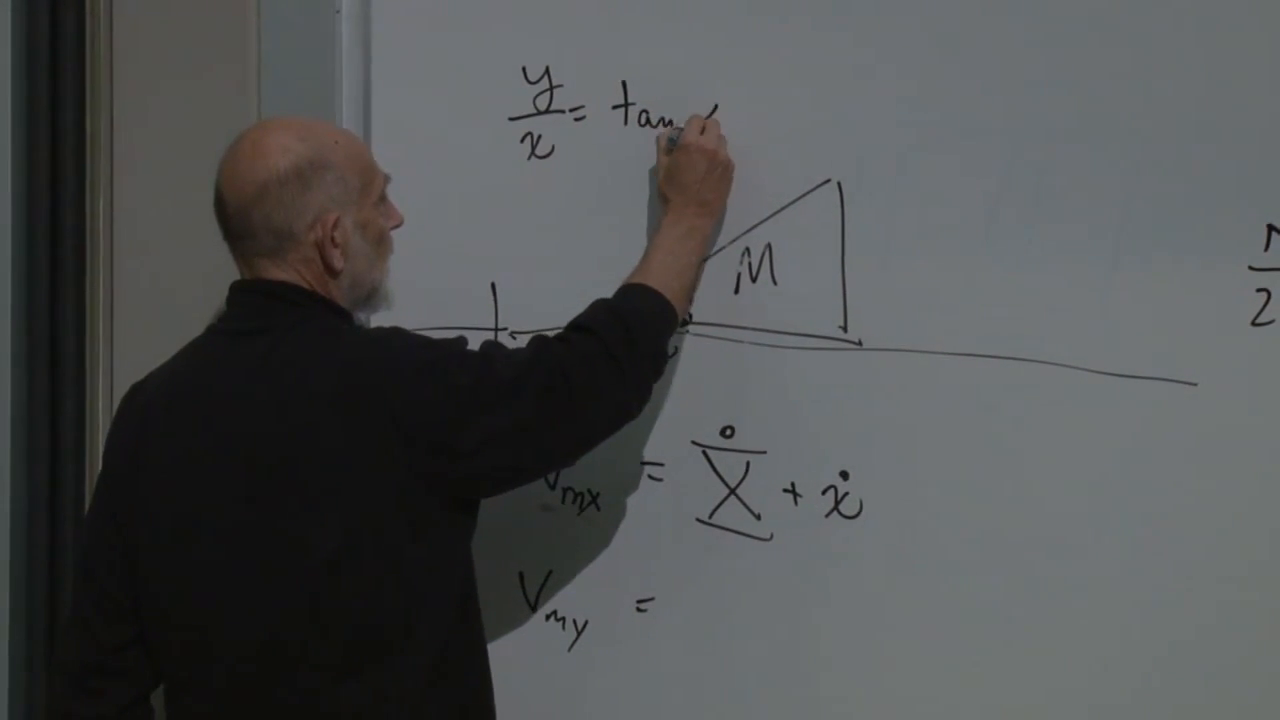
\includegraphics[width=0.84\textwidth]{lecture_06_figure_06.png}
  \caption{运动的楔块、受约束的质点，以及\(45^\circ\)例子中使用的水平和竖直速度分量。}
  \lectureframe{00:10:25}
\end{figure}

楔块的动能为
\begin{equation}
  T_{M}=\frac{M}{2}\dot X^2.
  \label{eq:l6-wedge-kinetic}
\end{equation}
质点的水平速度是\(\dot X+\dot x\)，而它的竖直速度是\(\dot x\)。因此它的动能为
\begin{equation}
  T_m=\frac{m}{2}\left[(\dot X+\dot x)^2+\dot x^2\right].
  \label{eq:l6-particle-kinetic}
\end{equation}
取\(x=0\)处为引力势能的零点，我们有\(V=mgx\)。因此
\begin{equation}
  L=\frac{M}{2}\dot X^2
    +\frac{m}{2}\left[(\dot X+\dot x)^2+\dot x^2\right]
    -mgx.
  \label{eq:l6-wedge-lagrangian}
\end{equation}

\begin{figure}[htbp]
  \centering
  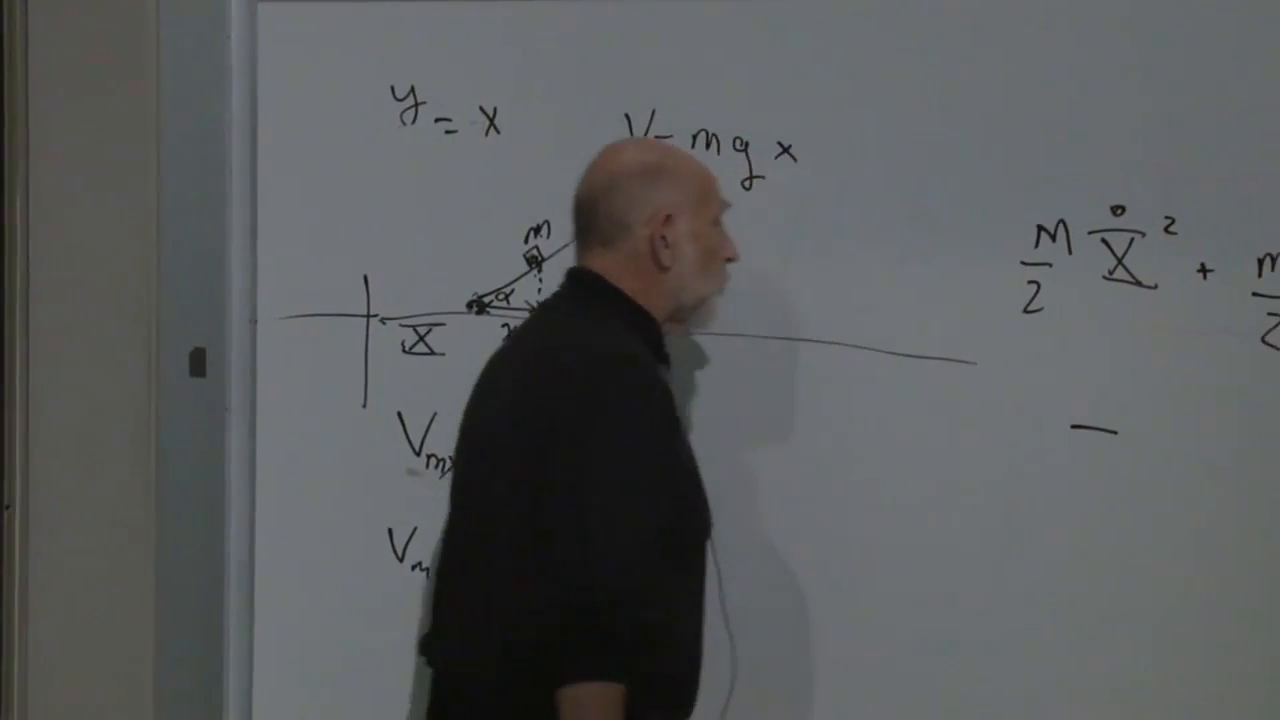
\includegraphics[width=0.86\textwidth]{lecture_06_figure_07.png}
  \caption{楔块的几何、\(V=mgx\)，以及两项动能贡献被汇集到黑板上。}
  \lectureframe{00:14:15}
\end{figure}

\subsection{正则动量由拉格朗日量定义}

正则动量由拉格朗日量定义，而不是由基于单个质点速度的猜测来定义：
\begin{align}
  p_X&=\frac{\partial L}{\partial\dot X}
      =M\dot X+m(\dot X+\dot x),
      \label{eq:l6-wedge-pX}\\
  p_x&=\frac{\partial L}{\partial\dot x}
      =m(\dot X+\dot x)+m\dot x.
      \label{eq:l6-wedge-px}
\end{align}
第一个表达式就是通常的总水平动量：楔块贡献\(M\dot X\)，质点贡献
\(m(\dot X+\dot x)\)。它在这里表现为与坐标\(X\)共轭的动量。

\begin{figure}[htbp]
  \centering
  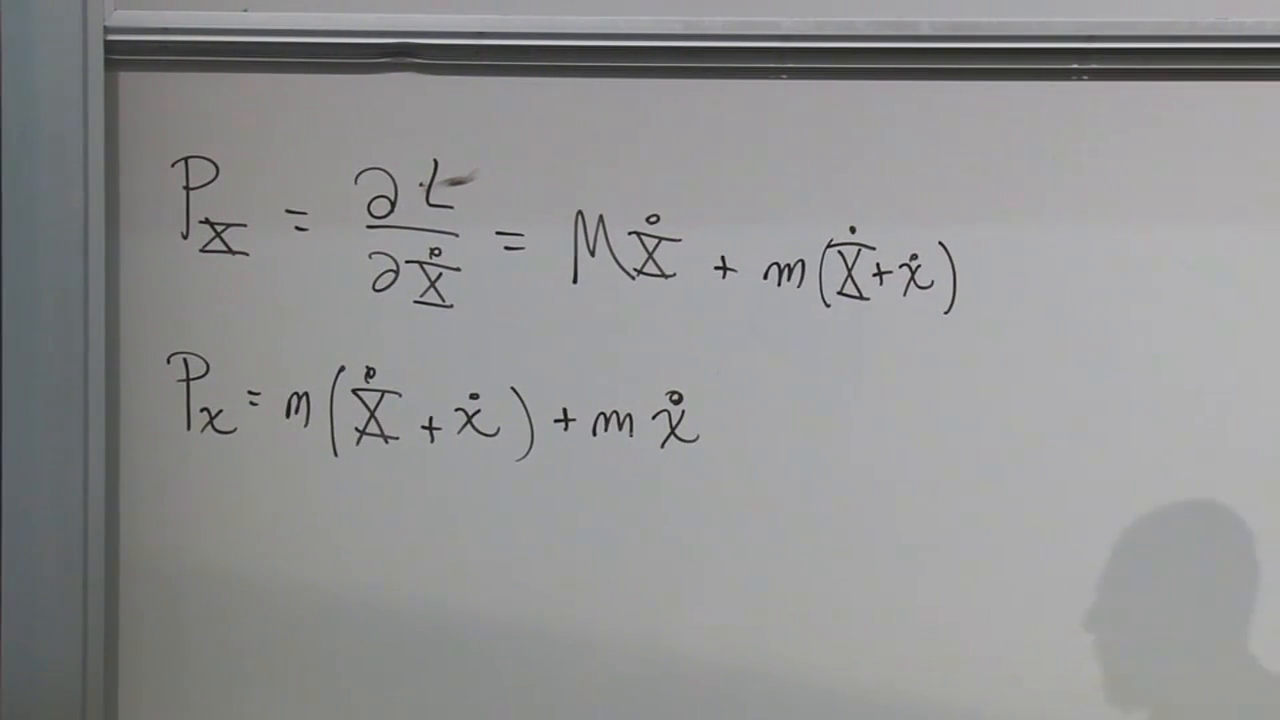
\includegraphics[width=0.86\textwidth]{lecture_06_figure_08.png}
  \caption{与楔块坐标\(X\)和质点相对坐标\(x\)共轭的正则动量。}
  \lectureframe{00:18:05}
\end{figure}

拉格朗日量不显含\(X\)。整个装置的平移表现为
\begin{equation}
  \delta X=\epsilon,
  \qquad
  \delta x=0.
  \label{eq:l6-wedge-translation}
\end{equation}
因此一般无穷小对称性规则
\begin{equation}
  \delta q_i=\epsilon f_i(q),
  \qquad
  Q=\sum_i p_i f_i
  \label{eq:l6-noether-rule}
\end{equation}
给出\(Q=p_X\)。等价地，\(X\)是循环坐标，且
\begin{equation}
  \dot p_X=\frac{\partial L}{\partial X}=0.
  \label{eq:l6-wedge-conservation}
\end{equation}

不存在相应的竖直平移对称性。楔块不允许竖直移动，而改变质点的高度会改变引力势能。水平动量守恒；这个受约束子系统的竖直动量不守恒。

对于相对坐标，欧拉--拉格朗日方程为
\begin{equation}
  \dot p_x=\frac{\partial L}{\partial x}=-mg.
  \label{eq:l6-wedge-force}
\end{equation}
这一行在板书上需要修正一个符号。可靠的途径是从\(L=T-V\)出发：由于\(V=mgx\)，拉格朗日量的导数为\(-mg\)。\(x\)是作为水平位移引入的，这一事实并不会把重力从它的方程中移除，因为约束把该水平位移与竖直高度\(y=x\)联系了起来。

没有出现任何法向力或约束反力。这类力就是维持约束所必需的任何值。牛顿方法会引入它们，并连同加速度一起求解；广义坐标使它们变得不必要。

\section{双摆与坐标的艺术}

现在把两个单位质量悬挂在两根单位长度的无质量杆上。第一根杆与竖直向下方向成角\(\theta\)。对于第二个自由度，我们有一个选择。我们可以使用第二个绝对角\(\phi\)，也可以使用两杆之间的相对角\(\alpha\)。

相对角是更具启发性的选择。暂时关闭重力。整个装置的刚性旋转会改变绝对取向，但不会改变两杆之间的夹角：
\begin{equation}
  \theta\longrightarrow\theta+\epsilon,
  \qquad
  \alpha\longrightarrow\alpha.
  \label{eq:l6-double-rotation}
\end{equation}
采用这一选择后，旋转对称性只作用在一个坐标上。这并不意味着其他坐标系是错的。它只是使对称性、从而也使守恒量更容易看出。

\begin{figure}[htbp]
  \centering
  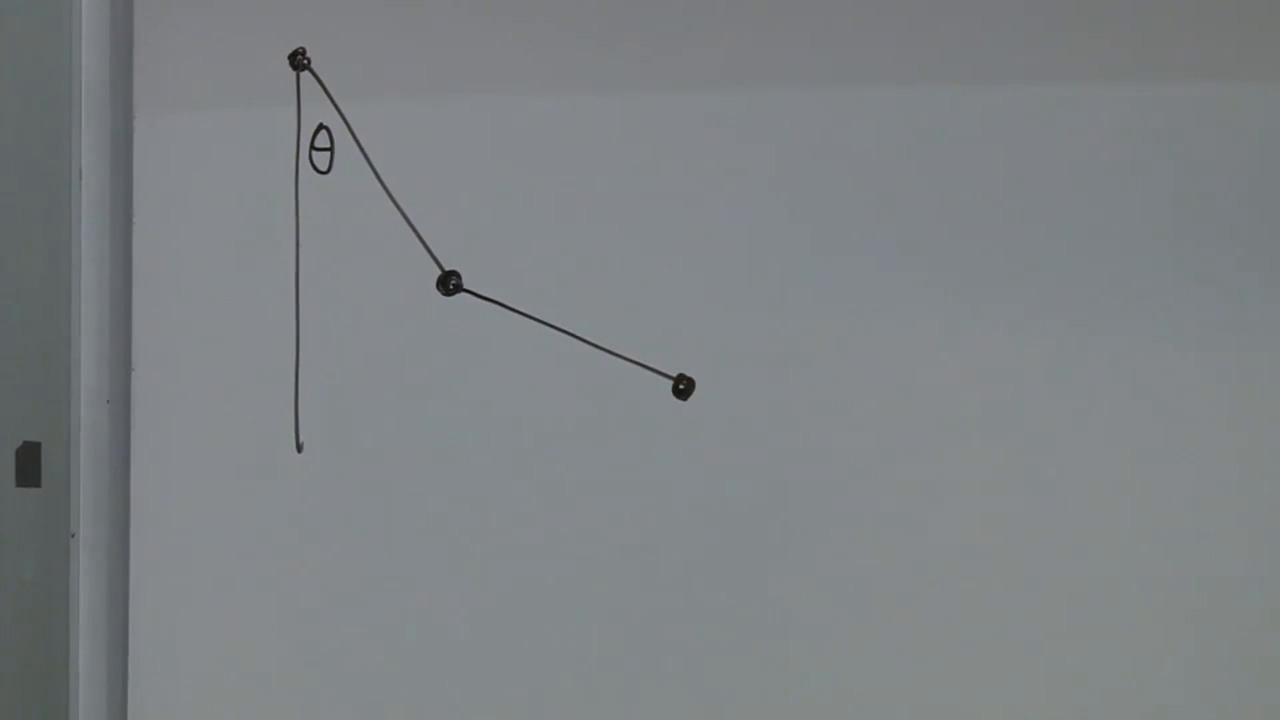
\includegraphics[width=0.76\textwidth]{lecture_06_figure_09.png}
  \caption{以\(\theta\)为第一个绝对角、\(\alpha\)为第二根杆相对于第一根杆的角的双摆。}
  \lectureframe{00:29:20}
\end{figure}

为得到动能，可把笛卡儿坐标用作临时的记账工具。取竖直坐标向下为正，第一个摆球位于
\begin{equation}
  x_1=\sin\theta,
  \qquad
  y_1=\cos\theta,
  \label{eq:l6-bob-one-position}
\end{equation}
因而
\begin{equation}
  \dot x_1=\dot\theta\cos\theta,
  \qquad
  \dot y_1=-\dot\theta\sin\theta,
  \qquad
  \dot x_1^2+\dot y_1^2=\dot\theta^2.
  \label{eq:l6-bob-one-velocity}
\end{equation}
第二个摆球位于
\begin{align}
  x_2&=\sin\theta+\sin(\theta+\alpha),\\
  y_2&=\cos\theta+\cos(\theta+\alpha),
  \label{eq:l6-bob-two-position}
\end{align}
所以，例如
\begin{equation}
  \dot x_2=\dot\theta\cos\theta
  +(\dot\theta+\dot\alpha)\cos(\theta+\alpha),
  \label{eq:l6-bob-two-xvelocity}
\end{equation}
而\(\dot y_2\)有类似的表达式。

\begin{figure}[htbp]
  \centering
  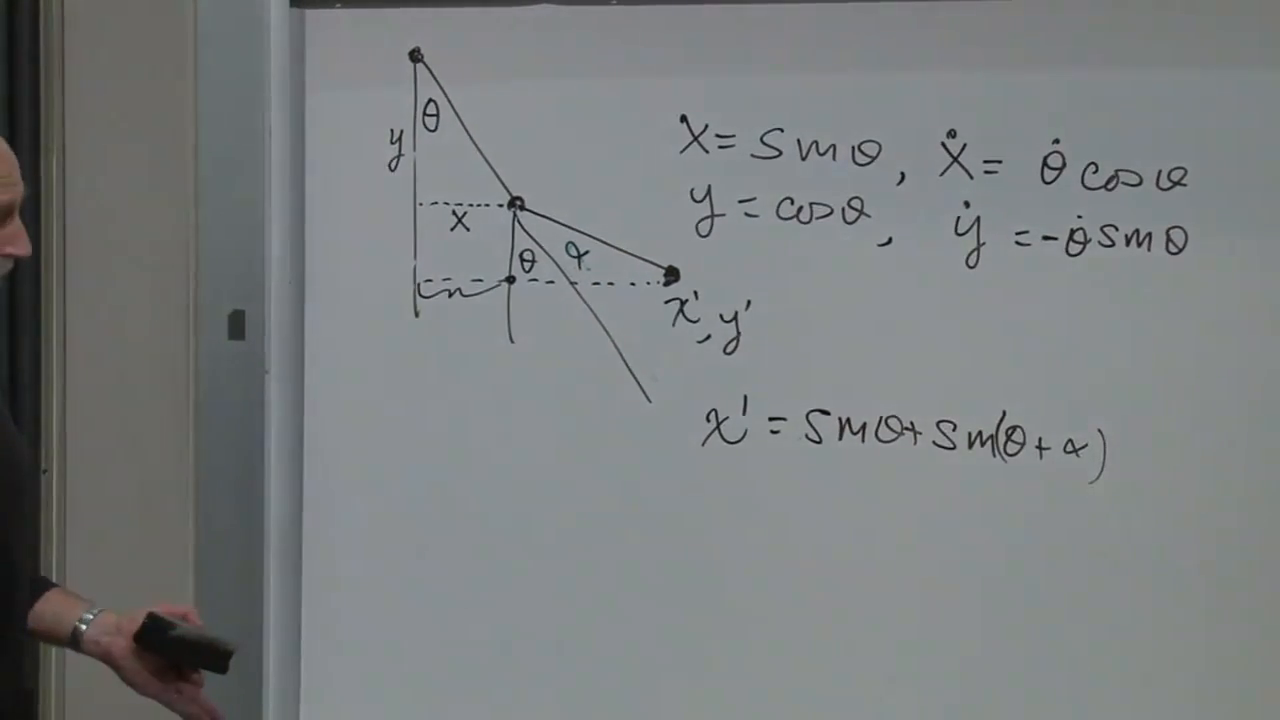
\includegraphics[width=0.88\textwidth]{lecture_06_figure_10.png}
  \caption{两个摆球的辅助笛卡儿坐标。它们用于计算速度，而不是作为额外的自由度引入。}
  \lectureframe{00:35:25}
\end{figure}

把两个动能相加，得到下面这个自洽的结果。交叉项来自
\begin{equation*}
  \cos A\cos B+\sin A\sin B=\cos(A-B).
\end{equation*}
\begin{equation}
  T=\dot\theta^2
    +\frac12(\dot\theta+\dot\alpha)^2
    +\dot\theta(\dot\theta+\dot\alpha)\cos\alpha.
  \label{eq:l6-double-kinetic}
\end{equation}

\begin{classroomqa}
  \audiencequestion{这个表达式是否已经包含两个摆球的动能，是否丢掉了一个二分之一因子？
  \lecturetimestamp{00:38:06--00:38:27}}
  \lecturerresponse{它包含两者。它来自
  \(\tfrac12(\dot x_1^2+\dot y_1^2+\dot x_2^2+\dot y_2^2)\)。
  两个相等的贡献合起来产生第一项\(\dot\theta^2\)；没有因子丢失。}
\end{classroomqa}

没有重力时，\(L=T\)不显含\(\theta\)。因此
\begin{equation}
  \dot p_\theta=\frac{\partial L}{\partial\theta}=0,
  \label{eq:l6-double-angular-conservation}
\end{equation}
而\(p_\theta\)就是总角动量。请注意“\(\theta\)不出现”这一说法的确切含义：\(\dot\theta\)当然会出现，但未微分的坐标不出现。

恢复重力会破坏整体旋转对称性。对于上面取竖直向下的约定，一种方便的零点选择给出
\begin{equation}
  V=-g(y_1+y_2)
   =-g\left[2\cos\theta+\cos(\theta+\alpha)\right].
  \label{eq:l6-double-potential}
\end{equation}
加上一个常数不会改变任何东西。要点在于\(\theta\)现在显式出现，因此它的共轭动量不再守恒。能量仍然守恒，因为拉格朗日量不显含时间。

\begin{classroomqa}
  \audiencequestion{板书上的\(\dot\theta-\dot\alpha\)是否应为\(\dot\theta+\dot\alpha\)？
  \lecturetimestamp{00:43:00--00:43:54}}
  \lecturerresponse{这里所用的取向要求正号。它是式~\eqref{eq:l6-bob-two-position}中的约定，并一直贯穿到式~\eqref{eq:l6-double-kinetic}中的动能。反转正\(\alpha\)的定义会改变相应的符号，但此后每一次出现都必须一致地改变。板书把两种约定混在了一起。}
\end{classroomqa}

\begin{figure}[htbp]
  \centering
  \includegraphics[width=0.84\textwidth]{lecture_06_figure_02.png}
  \caption{无重力摆的计算以及\(\dot p_\theta=\partial L/\partial\theta\)。上面一行板书保留了问题中讨论的符号不一致的局部记号；归一化后的公式是式~\eqref{eq:l6-double-kinetic}。}
  \lectureframe{00:45:50}
\end{figure}

一旦\(T\)和\(V\)已知，其余方程就通过微分得到。杆的张力以及维持长度固定的力再次消失在坐标的选择之中。

\subsection{守恒意味着什么、不意味着什么}

\begin{classroomqa}
  \audiencequestion{能否直接从方程看出双摆是混沌的？
  \lecturetimestamp{00:44:57--00:45:25}}
  \lecturerresponse{通常不能靠简单观察看出。随着参数或能量变化，系统可能从规则行为过渡到混沌行为。这个问题需要比方程的表面形式更多的结构，将在后面讨论。}
\end{classroomqa}

\begin{classroomqa}
  \audiencequestion{在保守系统中，是否每个\(\dot p_i\)都等于零？
  \lecturetimestamp{00:45:25--00:46:24}}
  \lecturerresponse{不是。一般方程为
  \(\dot p_i=\partial L/\partial q_i\)。只有当\(q_i\)是循环坐标时它才为零。循环坐标是一种特别简单的情形，其中通过对称性使一个坐标发生移动，而其余坐标保持不变。}
\end{classroomqa}

如果唯一的目标是数值演化，那么即使使用不方便的坐标系也仍然可行；它只是产生更长的方程。巧妙坐标系的回报是概念上的：在解方程之前，守恒的动量就已经可见。

\begin{classroomqa}
  \audiencequestion{在没有重力的情况下，双摆的行为是否像单个自由摆那样简单？
  \lecturetimestamp{00:47:02--00:47:35}}
  \lecturerresponse{单个自由转子匀速转动，因为它的一个角动量决定了它的运动。双摆可以执行非常复杂的相对运动，同时保持总角动量守恒。如果两个角速度初始时都为零，它就保持静止；否则，两部分会相互作用。}
\end{classroomqa}

\begin{classroomqa}
  \audiencequestion{在没有重力时，\(\dot\theta\)和\(\dot\alpha\)各自都是常量吗？
  \lecturetimestamp{00:47:36--00:52:42}}
  \lecturerresponse{不是。守恒说的是\(\dot p_\theta=0\)，而不是\(\ddot\theta=0\)或\(\ddot\alpha=0\)。\(p_\theta=\partial L/\partial\dot\theta\)的表达式包含两个角速度，并且依赖于\(\alpha\)。杆传递力矩，使两个摆锤能够交换角动量和能量。这类似于由弹簧连接的两个质量：总动量和质心速度是常量，而各个速度则振荡。其转动类比是一个特定的集体组合，而不是任何一个角度本身。}
\end{classroomqa}

\begin{classroomqa}
  \audiencequestion{交换角动量的力是通过杆传递的吗？
  \lecturetimestamp{00:52:43--00:53:34}}
  \lecturerresponse{是的。沿杆传递的力不必指向另一个运动的支点，因此它可以施加力矩。力矩不过是力的转动趋势，而在这里它产生了非零的各个角加速度。}
\end{classroomqa}

\section{作为第三种表述的哈密顿量}

哈密顿量就是能量，但这只是它的第一层意义。它也是力学第三种表述的基础。牛顿方程使用力和加速度。稳定作用量原理给出欧拉--拉格朗日方程。对于正则系统，哈密顿力学与后者等价，但它的变量和几何看起来不同。

不用\(q_i\)和\(\dot q_i\)，而使用\(q_i\)及其共轭动量\(p_i\)。具有\(n\)个自由度的系统的一个状态，在任一种描述中都需要\(2n\)个数：位置和速度，或者位置和动量。它们之间的桥梁是
\begin{equation}
  p_i=\frac{\partial L}{\partial\dot q_i}.
  \label{eq:l6-legendre-map}
\end{equation}
当这些关系可以对速度\(\dot q_i(q,p)\)求逆时，定义
\begin{equation}
  H(q,p)=\sum_i p_i\dot q_i-L(q,\dot q).
  \label{eq:l6-hamiltonian-definition}
\end{equation}
然后右端的速度被消去，改用\(q\)和\(p\)表示。这种可逆性就是正则勒让德变换的假设。奇异拉格朗日量需要更一般的约束理论；它们不由这种初等构造处理。

\subsection{微积分之前的可逆性}

回想一个由箭头连接的抽象状态的有限集合。如果两个较早的状态流入一个较晚的状态，那么确定性规则仍可能不可逆。未来是唯一的，但过去不是。把所有箭头反转，就得到相反的缺陷：一个状态分叉成多个未来。在第一幅图中箭头汇聚；在第二幅图中它们发散。

\begin{figure}[htbp]
  \centering
  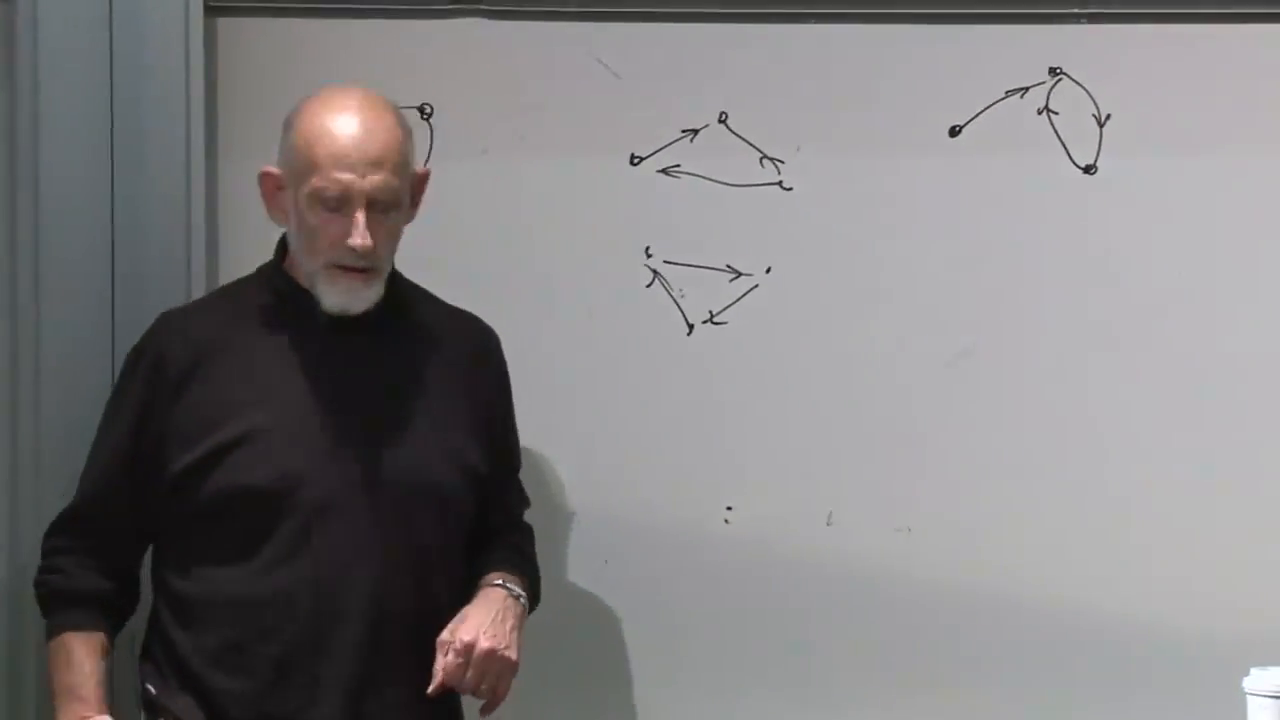
\includegraphics[width=0.86\textwidth]{lecture_06_figure_11.png}
  \caption{用于对比可逆循环与被禁止的汇聚和发散的抽象状态映射。}
  \lectureframe{00:56:20}
\end{figure}

哈密顿流将提供这一陈述的连续版本。一团相空间点可以移动和变形，但它不能获得一个破坏状态之间区别的汇，也不能获得一个从单个状态制造出多个未来的源。证明留待以后；目前这些图用于启发几何。

\begin{classroomqa}
  \audiencequestion{抽象状态图是否应被解释为在引力场中运动的物体？
  \lecturetimestamp{00:58:02--00:58:35}}
  \lecturerresponse{不是。这些点只是抽象状态，箭头规定了一条改变状态的规则。该图没有被赋予任何空间或引力意义。}
\end{classroomqa}

\begin{classroomqa}
  \audiencequestion{一个被禁止的收敛态映射如何与黑洞相区分？
  \lecturetimestamp{00:58:40--00:59:28}}
  \lecturerresponse{只能困难而微妙地做到。这是一个合理的问题，但正确的回答需要对完整状态及其量子引力演化进行细致的描述。仅凭基本图像不足以解决它。}
\end{classroomqa}

\section{一个适配相空间的振子}

在推导一般方程之前，考虑用刻意适配的变量写出的谐振子：
\begin{equation}
  L=\frac{1}{2\omega}\dot q^2-\frac{\omega}{2}q^2.
  \label{eq:l6-rescaled-lagrangian}
\end{equation}
其共轭动量为
\begin{equation}
  p=\frac{\partial L}{\partial\dot q}=\frac{\dot q}{\omega},
  \qquad
  \dot q=\omega p.
  \label{eq:l6-rescaled-momentum}
\end{equation}
代入式~\eqref{eq:l6-hamiltonian-definition}得
\begin{align}
  H&=p\dot q-L\\
   &=\omega p^2-\frac{\omega p^2}{2}+\frac{\omega q^2}{2}
    =\frac{\omega}{2}(p^2+q^2).
  \label{eq:l6-oscillator-hamiltonian}
\end{align}

\begin{figure}[htbp]
  \centering
  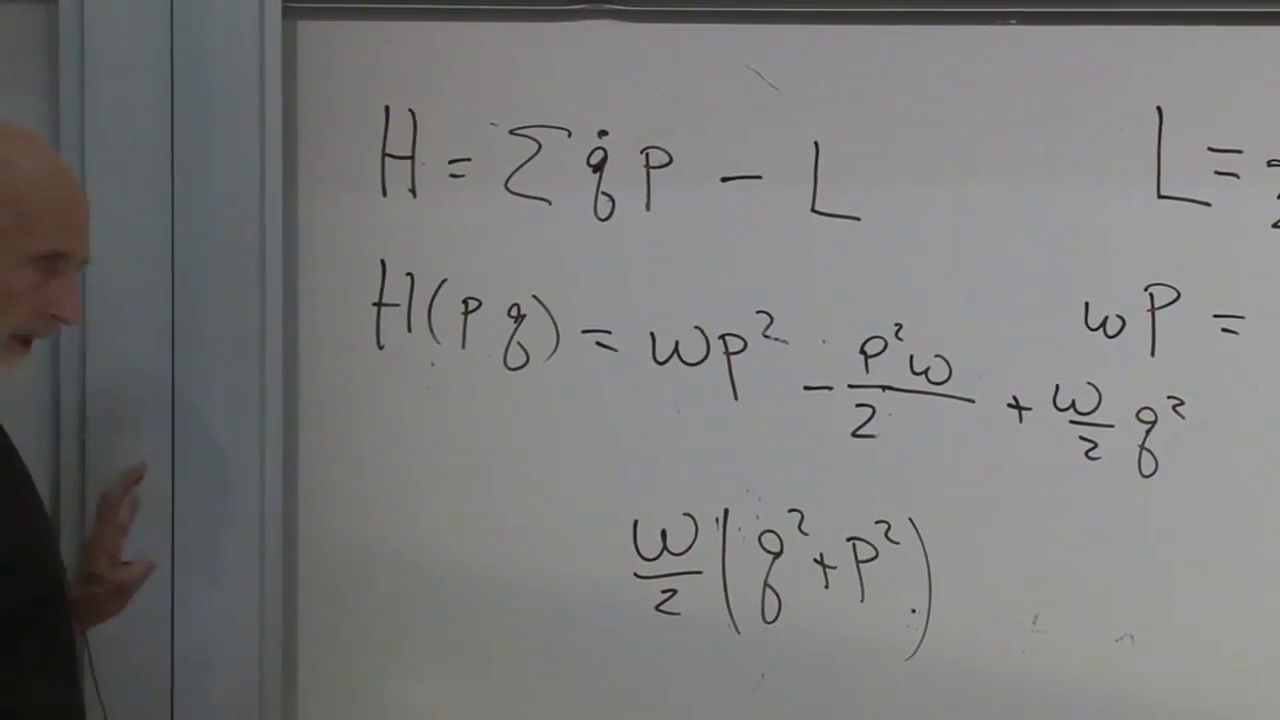
\includegraphics[width=0.86\textwidth]{lecture_06_figure_12.png}
  \caption{适配振子的勒让德变换与对称哈密顿量\(H=\tfrac{\omega}{2}(p^2+q^2)\)。}
  \lectureframe{01:08:20}
\end{figure}

\(q\)与\(p\)构成的空间是相空间。一个自由度给出二维平面；两个自由度给出四维相空间。在振子能量固定时，
\begin{equation}
  p^2+q^2=\frac{2H}{\omega},
  \label{eq:l6-energy-circle}
\end{equation}
因此轨迹保持在圆上。能量守恒将运动限制在这样一条曲线上。

\begin{figure}[htbp]
  \centering
  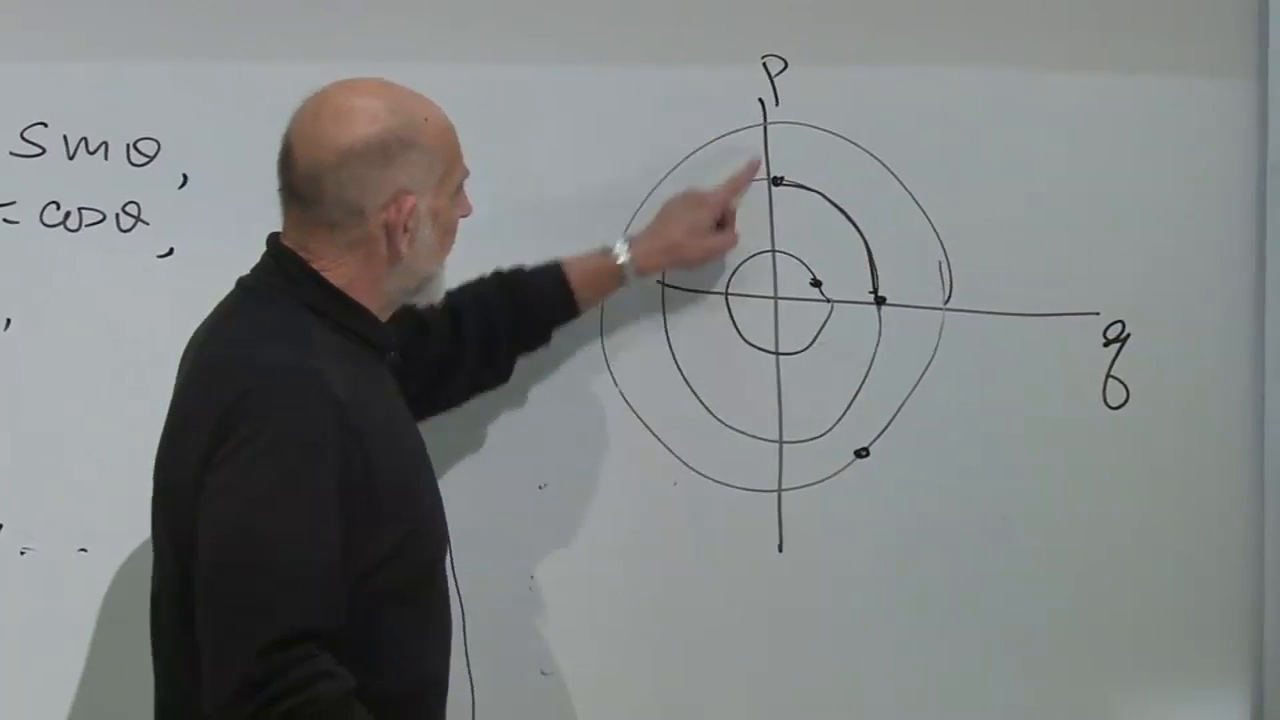
\includegraphics[width=0.82\textwidth]{lecture_06_figure_13.png}
  \caption{振子相平面中嵌套的等能圆，\(q\)为水平方向，\(p\)为竖直方向。}
  \lectureframe{01:13:20}
\end{figure}

\section{推导哈密顿方程}

这一推导是多元函数微分的一个练习。对于\(F(q,p)\)，
\begin{equation}
  \delta F=\sum_i\left(
  \frac{\partial F}{\partial q_i}\delta q_i
  +\frac{\partial F}{\partial p_i}\delta p_i\right).
  \label{eq:l6-total-differential}
\end{equation}
系数可以从两个方向读出：\(\delta q_i\)的系数是\(\partial F/\partial q_i\)，而\(\delta p_i\)的系数是\(\partial F/\partial p_i\)。

现在对\(H\)的定义表达式作变分：
\begin{align}
  \delta H
  &=\sum_i\left(\dot q_i\,\delta p_i
       +p_i\,\delta\dot q_i\right)-\delta L\\
  &=\sum_i\left(\dot q_i\,\delta p_i
       +p_i\,\delta\dot q_i
       -\frac{\partial L}{\partial q_i}\delta q_i
       -\frac{\partial L}{\partial\dot q_i}\delta\dot q_i\right).
  \label{eq:l6-vary-hamiltonian}
\end{align}
由于\(\partial L/\partial\dot q_i=p_i\)，两个\(\delta\dot q_i\)项相消。欧拉--拉格朗日方程给出\(\partial L/\partial q_i=\dot p_i\)，于是剩下
\begin{equation}
  \delta H=\sum_i\left(\dot q_i\,\delta p_i
                     -\dot p_i\,\delta q_i\right).
  \label{eq:l6-reduced-variation}
\end{equation}

\begin{figure}[htbp]
  \centering
  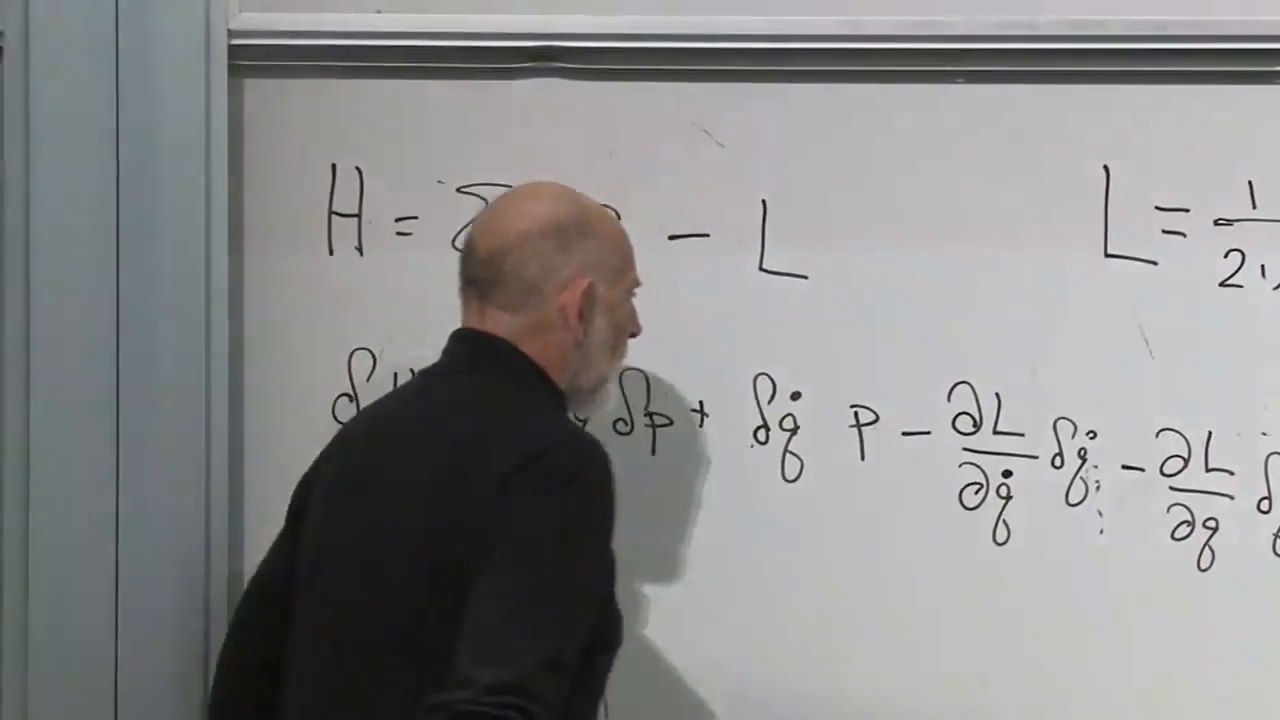
\includegraphics[width=0.86\textwidth]{lecture_06_figure_14.png}
  \caption{在\(p_i\,\delta\dot q_i\)项相消之前，\(\delta H\)的乘积法则展开。}
  \lectureframe{01:18:40}
\end{figure}

将式~\eqref{eq:l6-reduced-variation}与式~\eqref{eq:l6-total-differential}中的一般微分相比较，独立系数给出哈密顿方程：
\begin{equation}
  \boxed{
  \dot q_i=\frac{\partial H}{\partial p_i},
  \qquad
  \dot p_i=-\frac{\partial H}{\partial q_i}.}
  \label{eq:l6-hamilton-equations}
\end{equation}

\begin{figure}[htbp]
  \centering
  \includegraphics[width=0.78\textwidth]{lecture_06_figure_03.png}
  \caption{哈密顿量的定义、其变分以及加框的正则方程。}
  \lectureframe{01:22:18}
\end{figure}

对于\(n\)个坐标，这些是\(2n\)个一阶方程。欧拉--拉格朗日表述则给出\(n\)个二阶方程。初始数据的量与物理内容完全相同。

\section{作为刚性旋转的振子运动}

将式~\eqref{eq:l6-hamilton-equations}应用于式~\eqref{eq:l6-oscillator-hamiltonian}得
\begin{equation}
  \dot q=\omega p,
  \qquad
  \dot p=-\omega q.
  \label{eq:l6-oscillator-first-order}
\end{equation}
对第一个方程求导并利用第二个方程，
\begin{equation}
  \ddot q=\omega\dot p=-\omega^2q.
  \label{eq:l6-oscillator-second-order}
\end{equation}
因此这两个一阶方程恰好就是通常的二阶振子方程，连同动量的定义。

在相空间中，\((q,p)\)处的速度矢量为\((\dot q,\dot p)=(\omega p,-\omega q)\)，与能量圆相切。每个半径都以相同的角速度\(\omega\)旋转。整个平面可以被想象为一个刚性风车，或一种不可压缩的虚拟流体。它的点循环流动；它们既不会挤入一个汇，也不会从一个源飞散开。

\begin{figure}[htbp]
  \centering
  \includegraphics[width=0.86\textwidth]{lecture_06_figure_04.png}
  \caption{一团初始点分布在嵌套的相空间轨迹上。哈密顿演化移动这团点，而不是将其坍缩到一个偏好态中。}
  \lectureframe{01:39:27}
\end{figure}

\begin{figure}[htbp]
  \centering
  \includegraphics[width=0.90\textwidth]{lecture_06_figure_05.png}
  \caption{振子相图与等价的欧拉--拉格朗日方程\(\ddot q/\omega=-\omega q\)并列。}
  \lectureframe{01:42:10}
\end{figure}

下一步将把流体类比变成一个定理：哈密顿流没有局部收敛或发散。这一结果将连续力学与本课程开始时考虑的可逆态映射重新联系起来。

\section{揭示坐标选择的问题}

\begin{classroomqa}
  \audiencequestion{速度可以用\(q\)和\(p\)解出这一假设，是一个定理，还是物理系统的经验性质？
  \lecturetimestamp{01:29:08--01:29:45}}
  \lecturerresponse{在这一初等展开中，它是一个经验规律，其更深的动机来自量子力学。更确切地说，式~\eqref{eq:l6-legendre-map}关于速度必须具有非奇异雅可比矩阵。现代力学也包含重要的奇异拉格朗日量，尤其是约束系统和规范系统，但它们的哈密顿表述需要额外的约束机制。}
\end{classroomqa}

关于量纲的异议解释了为什么振子被写成式~\eqref{eq:l6-rescaled-lagrangian}那种不常见的形式。改为从普通坐标\(x\)出发：
\begin{equation}
  L=\frac{m}{2}\dot x^2-\frac{k}{2}x^2,
  \qquad
  \omega=\sqrt{\frac{k}{m}}.
  \label{eq:l6-ordinary-oscillator}
\end{equation}
选择
\begin{equation}
  q=(km)^{1/4}x.
  \label{eq:l6-oscillator-rescaling}
\end{equation}
于是\(q^2=\sqrt{km}\,x^2\)且\(\dot q^2=\sqrt{km}\,\dot x^2\)，这恰好把式~\eqref{eq:l6-ordinary-oscillator}化为式~\eqref{eq:l6-rescaled-lagrangian}。新的\(q\)是一个经过适配的广义坐标，而不是长度，其共轭量\(p\)也不是普通的力学动量\(p_x=m\dot x\)。

\begin{figure}[htbp]
  \centering
  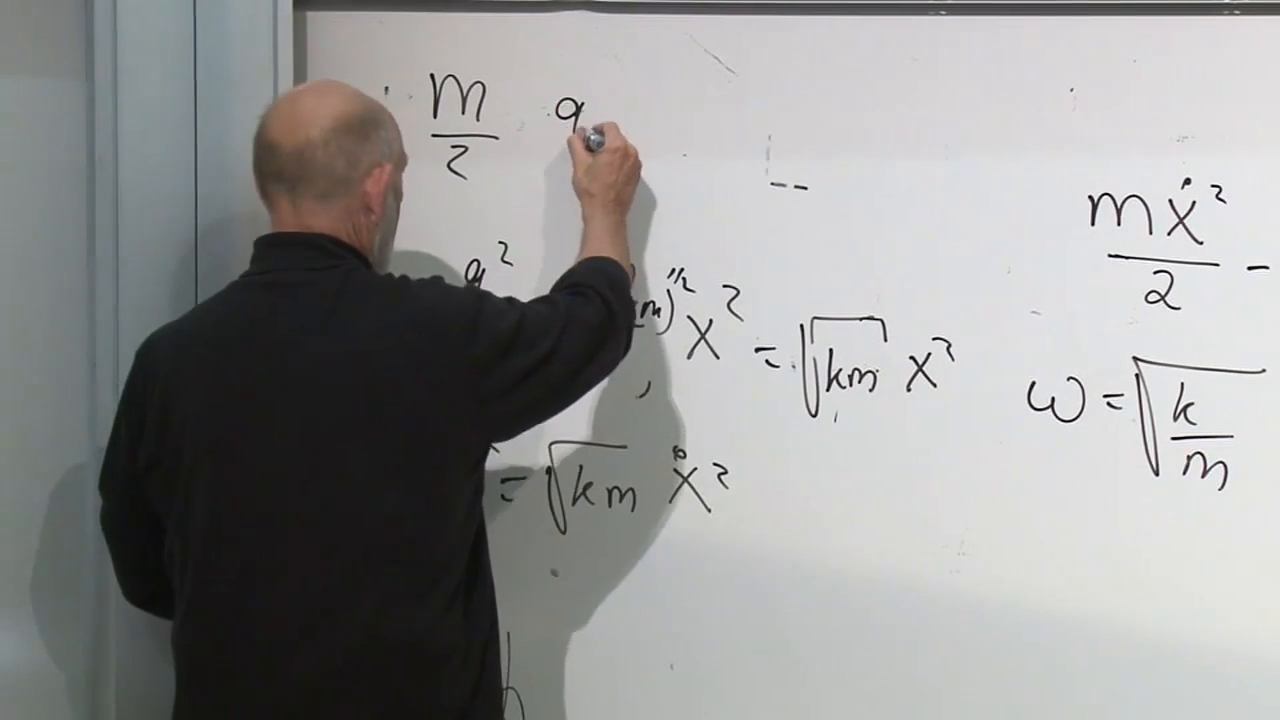
\includegraphics[width=0.86\textwidth]{lecture_06_figure_15.png}
  \caption{从通常的振子坐标\(x\)到适配坐标\(q=(km)^{1/4}x\)的量纲重标度。}
  \lectureframe{01:36:10}
\end{figure}

\begin{classroomqa}
  \audiencequestion{\(\omega p=\dot q\)怎么可能在量纲上自洽，又为什么要选择这些变量？
  \lecturetimestamp{01:29:46--01:39:22}}
  \lecturerresponse{符号\(q\)并不要求具有长度的量纲，其共轭量\(p\)也不要求具有\(m\dot x\)的量纲。式~\eqref{eq:l6-oscillator-rescaling}中的重标度保持了拉格朗日的量纲，并使\(q\)和\(p\)对称地进入\(H\)。在原来的变量中，
  \[
    H=\frac{p_x^2}{2m}+\frac{kx^2}{2},
  \]
  所以\((x,p_x)\)平面上的等能曲线是椭圆。在适配的\((q,p)\)平面上它们则是圆。选择这种重标度正是为了使该对称性显现出来。}
\end{classroomqa}

\begin{classroomqa}
  \audiencequestion{\(2n\)个一阶哈密顿方程怎么可能等价于\(n\)个二阶拉格朗日方程？
  \lecturetimestamp{01:39:24--01:42:30}}
  \lecturerresponse{对于振子，对\(\dot q=\omega p\)求导并代入\(\dot p=-\omega q\)；这一对方程变为\(\ddot q=-\omega^2q\)。直接从拉格朗日量出发则得到
  \[
    \frac{d}{dt}\left(\frac{\dot q}{\omega}\right)
      =-\omega q,
  \]
  这是同一个二阶方程。一个哈密顿方程可以看作由速度定义动量，而另一个则演化该动量。}
\end{classroomqa}

\section{为什么相空间与势能重要}

\begin{classroomqa}
  \audiencequestion{哈密顿量的威力是否意味着相空间是比位形空间更好的几何表示？
  \lecturetimestamp{01:42:33--01:44:38}}
  \lecturerresponse{它们服务于不同的目的。相空间使循环、等能面以及不存在汇聚或发散这一点变得格外透明。对于其他问题，位形空间可能更好。强调\(H\)的更深刻原因在于，它在量子力学中成为一个核心且更直观的对象，而量子力学正是这门力学所指向的现代学科之一。}
\end{classroomqa}

\begin{classroomqa}
  \audiencequestion{势能是否应被视为力的积分？
  \lecturetimestamp{01:44:40--01:45:45}}
  \lecturerresponse{对于保守力，这一说法成立，但相差一个常数，并且符号要取适当。更有用的方向是把势能视为基本的，并由它导出广义力：
  \[
    F_i=-\frac{\partial V}{\partial q_i}.
  \]
  当\(L=T-V\)且动能不显含\(q_i\)时，这正是出现在\(\dot p_i=\partial L/\partial q_i\)中的那一项。}
\end{classroomqa}

\begin{classroomqa}
  \audiencequestion{这条通向现代物理学的道路意在阐明哪些前沿问题？
  \lecturetimestamp{01:45:46--01:47:47}}
  \lecturerresponse{这条道路通向量子引力与宇宙学；基本粒子物理，包括希格斯部分和中微子；相对论；弦论；以及量子场论。持久的理论问题在于把这些片段纳入一个连贯的结构，尤其是把量子力学与引力、把宇宙学与粒子物理结合起来。这是对2011年时前沿状况的陈述，而不是声称其解决方案当时已经已知。}
\end{classroomqa}

这两个受约束的例子和振子现在被纳入同一幅图景。广义坐标去除了不必要的力。对称性选出守恒的正则动量。勒让德变换把速度换成动量，而哈密顿方程把动力学变成相空间上的流动。对于振子，该流动是刚性旋转；对于一般系统，其几何将给出可逆运动的精确连续含义。